\section{Source images}
As shown in Fig.\ref{fig:6.1}, source images grouped into three categories are employed to verify the effectiveness of the proposed fusion framework. Among them, there are  multi-focus images Figs.\ref{fig:6.1},visible-infrared images Fig. \ref{fig:6.1}
and  medical images \ref{fig:6.1}. For each pair, the two
source images are assumed to be pre-registered in our study.

\begin{figure}[h!]
  \centering
  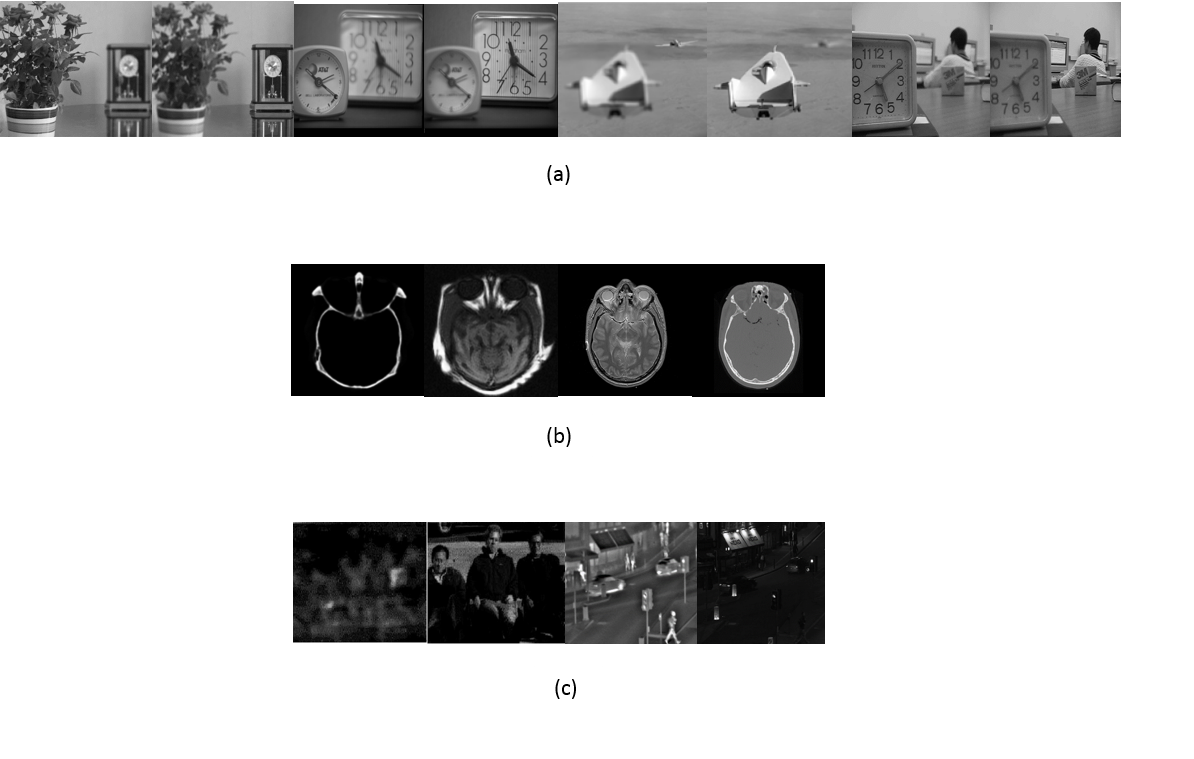
\includegraphics[width=1\textwidth]{sources.png}
  \caption{The source images used in our experiments. (a) Multi-focus images,(b)medical images   and (c) visible-infrared images} \label{fig:6.1}
\end{figure}

\section{Objective evaluation metrics}
It is not an easy task to quantitatively evaluate the quality of a fused image since the reference image (ground truth) does not
exist in practice. In recent years, many fusion metrics have been
proposed, but none of them is universally believed to be always
more reasonable than others for various fusion scenarios. Thus, it is usually necessary to apply several metrics to make a comprehensive evaluation. In this work, five popular metrics, which are briefly introduced as follows, are employed to quantitatively evaluate the performances of different fusion methods. Uniformly, let A and B denote two source images of size \( H \times W \)while F represents the fused image.The different metrics are

\begin{itemize}
\item Standard deviation (SD). The SD of the fused image is defined as 
 \begin{equation}
 SD=\sqrt{\frac{1}{ H \times W}\sum_{x=1}^{H}\sum_{y=1}^{w} {\left(F\left(x,y \right) -\mu \right)}{^2}}
 \end{equation}
 where \(\mu\) is the mean value
\item  \textbf{Entropy (EN)} The EN of the fused image is defined as
\begin{equation}
EN=-\sum _{l=0}^{L-1}P_{F}\left(l \right)log_{2}{P}_{F}\left(l \right)
\end{equation}
where L is the number of gray level and \(P_{F} \)
is the normalized histogram of the fused image. In our experiments,L is set to 256.EN is used to measure the amount of information in the fused image
\item  The gradient based fusion metric \(Q_{G}\) proposed by Xydeas and Petrovic[23]. It is calculated by
\begin{equation}
Q_{G}=\frac{\sum _{x=1}^{H}\sum _{y=1}^{W}\left(Q^{AF}\left(x,y \right)W^{A} \left(x,y \right)+Q^{BF}\left(x,y \right)W^{B}\left(xx,y \right)\right)}{\sum _{x=1}^{H}\sum_{y=1}^{W}\left(W^{A}\left(x,y \right)+W^{B}\left(x,y \right) \right) }
\end{equation}
 The \(Q_{G}\) is a popular
fusion metric which computes the amount of gradient information injected into the fused image from the source images
\item \textbf{PSNR } can reflect the quality of reconstruction. The larger the PSNR
is, the less the image distortion is.
\begin{equation}
PSNR=10 log\left(255^{2}/MSE\right)
\end{equation}

\item  \textbf{Structural similarity (SSIM)} Given the two source images X(X=a  orb)and the fused image f,the size of the images are all M×N, let X and f denote the mean of X, f, let \(\sigma_{x}^{2}\)and \(\sigma_{Xf}\) be the variance of X and covariance of X,f, respectively,
\begin{equation}
\sigma _{x}^{2}=\frac{1}{MN-1}\sum_{m=1}^{M} \sum_{n=1}^{N}{\left(X\left(m,n \right)-\bar{X} \right)}^{2} 
\end{equation}
\begin{equation}
\sigma _{xf}=\frac{1}{MN-1}\sum_{m=1}^{M} \sum_{n=1}^{N}\left(X\left(m,n \right)-\bar{X} \right) \left(f\left(m,n \right) -\bar{f}\right)
\end{equation}

Since image signals are generally non-stationary, it is appropriate to measure the number \(Q_{0}\)over local regions and then combine the different results into a single measure. A sliding window w is used in the images.\(Q_{0}(x,f|w)\))is computed in each window. Then compute the whole image metric \(Q_{0}(x,f)\)

\end{itemize}




